%% !TEX root = manual.tex

\section{Network Topologies and Routing}
\label{sec:tutorial:topology}
We here give a brief introduction to specifying different topologies and routing strategies.  
We will only discuss one basic example (torus).  
A more thorough introduction covering all topologies is planned for future releases.
Excellent resources are ``Principles and Practices of Interconnection Networks'' by Brian Towles and William Dally published by Morgan Kaufman and ``High Performance Datacenter Networks'' by Dennis Abts and John Kim published by Morgan and Claypool.

\subsection{Topology}
\label{subsec:tutorial:topology}

Topologies are determined by two mandatory parameters.

\begin{ViFile}
topology.name = torus
topology.geometry = 4 4
\end{ViFile}
Here we choose a 2D-torus topology with extent 4 in both the $X$ and $Y$ dimensions for a total of 16 nodes (Figure \ref{fig:torus:basic})
The topology is laid out in a regular grid with network links connecting nearest neighbors.  
Additionally, wrap-around links connect the nodes on each boundary.  
\begin{figure}[h]
\centering
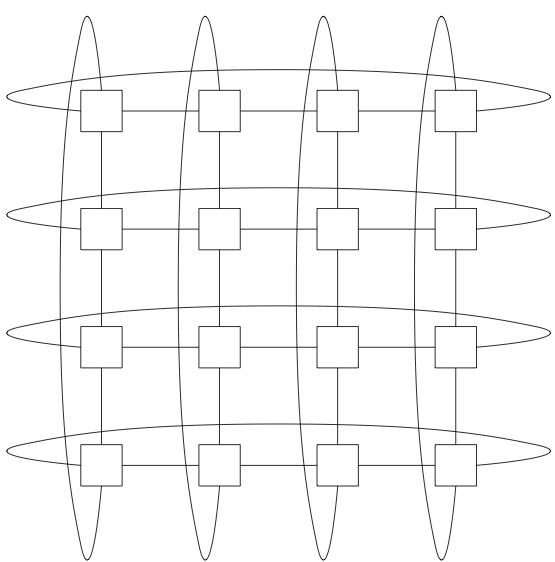
\includegraphics[width=0.5\textwidth]{figures/tikz/torus/torus.png}
\caption{4 x 4 2D Torus}
\label{fig:torus:basic}
\end{figure}


The figure is actually an oversimplification.  
The \inlinefile{topology_geometry} parameter actually specifies the topology of the \emph{network switches}, not the compute nodes. 
A torus is an example of a direct network in which each switch has one or more nodes ``directly'' connected to it.  
A more accurate picture of the network is given in Figure \ref{fig:torus:withnodes}.
\begin{figure}[h]
\centering
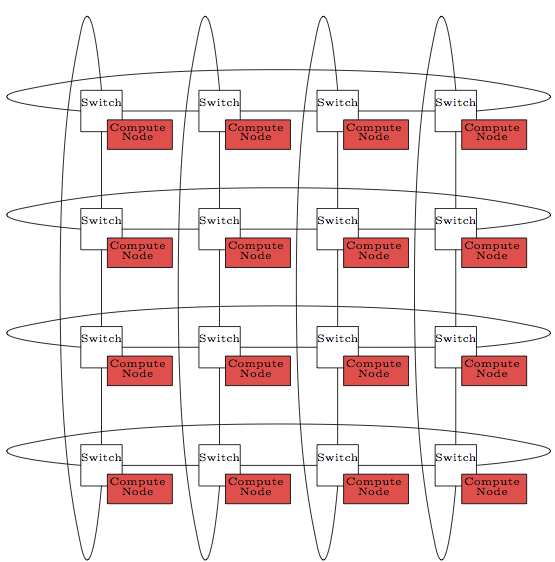
\includegraphics[width=0.4\textwidth]{figures/tikz/torus/withnodes.png}
\caption{4 x 4 2D Torus of Network Switches with Compute Nodes}
\label{fig:torus:withnodes}
\end{figure}
While in many previous architectures there was generally a one-to-one correspondence between compute nodes and switches, more recent architectures have multiple compute nodes per switch (e.g. Cray Gemini with two nodes).  
Multinode switches can be specified via

\begin{ViFile}
topology.name = torus
topology.geometry = 4 4
topology.concentration = 2
\end{ViFile}
which would now generate a torus topology with 16 switches and 32 compute nodes.

Another subtle modification of torus (and other networks) can be controlled by giving the $X$, $Y$, and $Z$ directions different bandwidth.  
The above network could be modified as

\begin{ViFile}
topology.name = torus
topology.geometry = 4 4
topology.redundant = 2 1
\end{ViFile}
giving the the $X$-dimension twice the bandwidth of the $Y$-dimension.  
This pattern DOES exist in some interconnects as a load-balancing strategy.  
A very subtle point arises here. Consider two different networks:

\begin{ViFile}
topology.name = torus
topology.geometry = 4 4
topology.redundant = 1 1
network_bandwidth = 2GB/s
\end{ViFile}
\begin{ViFile}
topology.name = torus
topology.geometry = 4 4
topology.redundant = 2 2
network_bandwidth = 1GB/s
\end{ViFile}
For some coarse-grained models, these two networks are exactly equivalent.  
In more fine-grained models, however, these are actually two different networks.  
The first network has ONE link carrying 2 GB/s. The second network has TWO links each carrying 1 GB/s.

\subsection{Routing}
\label{subsec:tutorial:routing}
By default, \sstmacro uses the simplest possible routing algorithm: dimension-order minimal routing (Figure \ref{fig:torus:basicrouting}).
\begin{figure}[h]
\centering
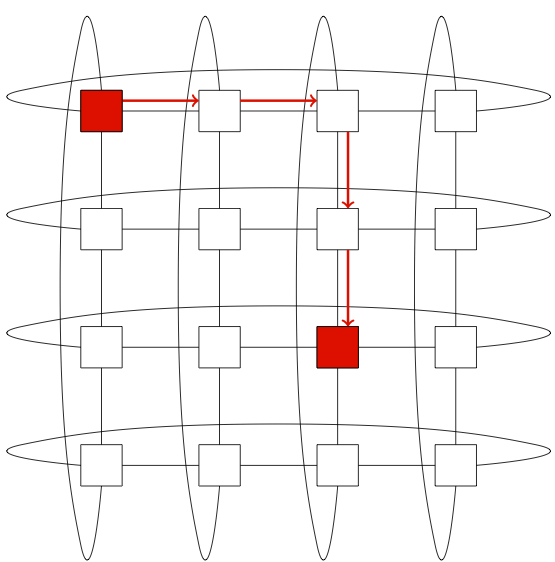
\includegraphics[width=0.4\textwidth]{figures/tikz/torus/minroutetorus.png}
\caption{Dimension-Order Minimal Routing on a 2D Torus}
\label{fig:torus:basicrouting}
\end{figure}
In going from source to destination, the message first travels along the $X$-dimension and then travels along the $Y$-dimension.
The above scheme is entirely static, making no adjustments to avoid congestion in the network.  
\sstmacro supports a variety of adaptive routing algorithms.  This can be specified:

\begin{ViFile}
router = min_ad
\end{ViFile}
which specifies minimal adaptive routing. 
There are now multiple valid paths between network endpoints, one of which is illustrated in Figure \ref{fig:torus:minadrouting}.
\begin{figure}[h!]
\centering
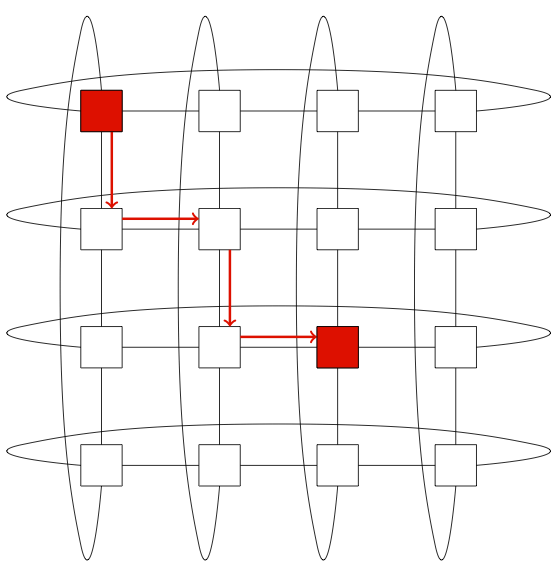
\includegraphics[width=0.4\textwidth]{figures/tikz/torus/minadroutetorus.png}
\caption{Adaptive Minimal Routing on a 2D Torus}
\label{fig:torus:minadrouting}
\end{figure}
At each network hop, the router chooses the \emph{productive} path with least congestion.  
In some cases, however, there is only one minimal path (node $(0,0)$ sending to $(2,0)$ with only $X$ different).
For these messages, minimal adaptive is exactly equivalent to dimension-order routing.  
Other supported routing schemes are valiant and UGAL.  More routing schemes are scheduled to be added in future versions.  
A full description of more complicated routing schemes will be given in its own chapter in future versions. 
For now, we direct users to existing resources such as ``High Performance Datacenter Networks'' by Dennis Abts and John Kim.
